
\section{同期・測距・校正手法のための制御システム}
同期のためには複数の端末がパルスを出し合わなければならないが,
いつどの端末がパルスを出すのか,といったスケジューリングをどうするかについて述べる(図\ref{fig:TDMA}).

\begin{figure}[p]\centering
  \hspace{-2mm}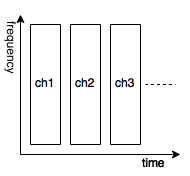
\includegraphics[clip,width=1.1\hsize]{img/TDMA.png}
  \caption{TDMA}\label{fig:TDMA}
\end{figure}

図\ref{fig:network2}にシステム全体のネットワーク構成を示す.

\begin{figure}[p]\centering
  \hspace{-2mm}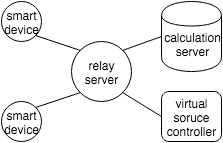
\includegraphics[clip,width=1.1\hsize]{img/network2.png}
  \caption{ネットワーク構成}\label{fig:network2}
\end{figure}

基本的には端末間の通信を中継するリレーサーバを中心としたスター型ネットワークである.
また,スピーカアレイに参加しない特別なノードとして,
計算用ノードと仮想音源を設定する制御用ノードがある.


今回の実装では中継サーバが同期アルゴリズムを制御している.
すべてのコマンドはリクエスト-レスポンスで成り立っており,リクエストを受けた端末は必ずレスポンスを返さねばならない.
まず,中継サーバはスピーカアレイを構成する端末に対して ping コマンドを送信し,
アレイに参加できる端末を確認する.
次に,全端末に対して録音をするように beginRec コマンドを送信する.
そして,各端末の放つパルスが排他的になるように,
パルスを放つ端末ごとにstartPulse,beepPulse,stopPulseコマンドを繰り返し送信する.
startPulseとstopPulseコマンドは,
この時間区間内にいずれかの端末からパルスが発信されることを示すもので,
後にパルス位置を検出するときの計算量を減らすためのコマンドである.
beepPulseは任意の一台の端末に対して,パルスを送信するように促すコマンドである.
すべての端末が互いに排他的にパルス発生し終えると,
最後にstopRecという録音終了コマンドを送信する.
その後,collectコマンドで各端末が録音したデータを集計し,
計算用サーバへ送信する(図\ref{fig:pulsediagram}).
計算用サーバは,それぞれの端末間のパルスの受信時刻を
先述の手法で検出し,相対信号伝達時間と相対距離計測,空間配置推定する.
その後,それらの情報を中継サーバを介して制御用端末へ送信する.




\begin{figure*}[p]\centering
\hspace{-2mm}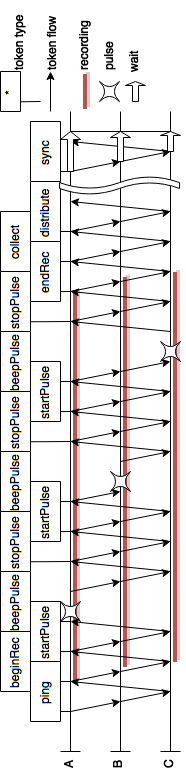
\includegraphics[clip,height=1.5\hsize]{img/flowchart.png}
\caption{システム動作のダイアグラム}\label{fig:pulsediagram}
\end{figure*}


\section{仮想音源配置によるDBAPアレイスピーカ制御システム}

仮想音源を配置し制御するための端末のユーザインターフェースを示す(図\ref{fig:relpos}).

\begin{figure}[p]\centering
  \hspace{-2mm}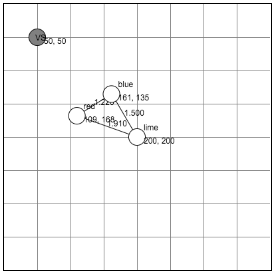
\includegraphics[clip,width=1.1\hsize]{img/relpos.png}
  \caption{仮想音源配置ユーザインタフェース}\label{fig:relpos}
\end{figure}

図のように推定した端末の分布図と,仮想音源を表示する.
仮想音源VSをドラッグすることで,DBAP法によって出力する振幅を計算し,各端末へ振幅を配信することで音像定位する.
また,音を鳴らしながら音源を移動させることも可能である.
